\section{Blocks Without Evidence}
\label{sec:evidence}

\subsection{Most blocks a policy can see are dead}
\label{sec:dead}
At the midpoint split, \textbf{92.8\% and 95.0\%} of the blocks visible on the conversation and toolagent
traces are never read again, and 88.8--96.0\% across splits from 0.3 to 0.7 (64.4\% on the synthetic
control). The few that are read again, 7{,}248 and 4{,}901 blocks, carry 45.7\% and 74.5\% of the
billable post-split reuse, and new blocks the rest, 54.3\% and 25.4\%. A policy that places blocks by
their prefix counts therefore fills the fast tiers mostly with blocks that will not be used, ahead of the
blocks it has not seen yet. Dead and new blocks alike give a split-time policy no evidence of future use:
a count that will not grow, or no count at all.

\subsection{The reference is set by a tie rule}
\label{sec:ties}
A natural reference for split-time policies gives every visible block its true future count and every
new block zero, and places them greedily~(\Cref{sec:defs}). Its dead visible blocks also get zero, and
which of two zero-belief blocks goes first is a tie rule. A stable sort in item order puts every visible
block ahead of every new one, and the reference then reaches 20.4\% and 15.3\% of the oracle's advantage
with tier-only actions (15.6\% and 12.4\% with all actions), which reads as most of the advantage being
out of a split-time policy's reach, the conclusion an earlier version of this paper drew and that we
retract (\Cref{sec:lessons}). Parking the dead blocks behind the new ones instead costs them
nothing --- they are never read --- and the same reference reaches:

\begin{center}\footnotesize\setlength{\tabcolsep}{3.5pt}
\begin{tabular}{@{}lrrr@{}}
\toprule
reference (tier-only actions) & conv. & tool. & synth. \\
\midrule
dead visible blocks ahead of new ones & 20.4 & 15.3 & 60.2 \\
dead visible blocks behind new ones & \textbf{77.8} & \textbf{76.2} & 84.1 \\
\midrule
same, all actions & 15.6 / 50.8 & 12.4 / 49.4 & 45.4 / 62.7 \\
\bottomrule
\end{tabular}
\end{center}
\noindent{\footnotesize Percent of the oracle's advantage over the frequency heuristic, split 0.5.}

\begin{figure}[t]
  \centering
  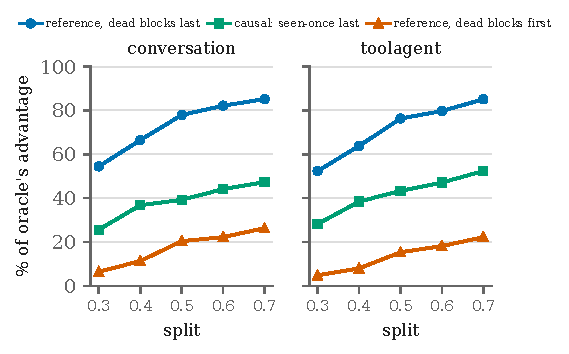
\includegraphics[width=\columnwidth]{fig_ties.pdf}
  \caption{The same clairvoyant split-time reference under the two tie rules for blocks without
  evidence, and the causal rule that parks seen-once blocks behind new ones, across splits (tier-only
  actions). The tie rule moves the reference by 48--63 points.}
  \label{fig:ties}
\end{figure}

\medskip
\noindent With tier-only actions the rule moves the reference by 48--63 points across splits on the
production traces, and by 30--72 points when the three bounded tiers are scaled together from a quarter
to one and a half times their sizes; the swing is smallest at the smallest tiers, where the reference
with dead blocks last reaches only 53--56\% (the synthetic control moves by 0--40 points). In serving
units, under the declared latencies the oracle's advantage is 32.6 and 16.2\,ms of block reads per
request after the split, so the rule moves the reference by 18.7 and 9.9\,ms per request.

The rule decides how a result reads. The strongest ranker of \Cref{sec:capacity}, an MLP trained with
all actions, gains 8.2\% and 7.4\% of the oracle's advantage: 52.6\% and 59.5\% of the way to the
reference with dead blocks first, a learned model past halfway to what looks reachable, but 16.2\% and
14.9\% of the way to the reference with them last.

Neither reference is an upper bound for the policies it stands for: on 200 random ten-block workloads an
exhaustive search over placements of the visible blocks beats the dead-first reference in 90 and the
dead-last one in 83, by reserving fast slots for arrivals, which needs knowledge of the arrivals. Knowing
only the arrivals' average does not lift the reference on the production traces: parking every visible
block whose future is below the mean future of the new blocks (0.35 and 0.34 accesses) parks exactly the
dead ones there, so the dead-last reference is already the one a split-time policy can build from the
arrival distribution. On the small workloads the average does help: the same rule closes 52.4\% of the gap
between the dead-last reference and the exhaustive search. We therefore report both references and call
neither a ceiling.

\subsection{Knowing which seen blocks are dead is most of the prize}
\label{sec:ladder}
Separating what the oracle knows into parts, each billed at the true cost (tier-only, split 0.5; the
last three rows are clairvoyant):

\begin{center}\footnotesize\setlength{\tabcolsep}{3.5pt}
\begin{tabular}{@{}lrrr@{}}
\toprule
& conv. & tool. & synth. \\
\midrule
frequency heuristic & 0.0 & 0.0 & 0.0 \\
\emph{causal:} seen-once behind new & 39.2 & 43.3 & 15.4 \\
\emph{causal:} estimated prior & 47.0 & 51.7 & 0.0 \\
which visible blocks are dead & 77.8 & 76.2 & 67.0 \\
visible futures, dead last & 77.8 & 76.2 & 84.1 \\
oracle & 100 & 100 & 100 \\
\bottomrule
\end{tabular}
\end{center}

\medskip
\noindent On the production traces, knowing only \emph{which} visible blocks are dead is worth as
much as knowing every visible block's future, to the hundredth of a point: the live visible blocks are few enough that their order
does not matter. What remains, 22--24\%, is the order among new blocks. The prefix approximates deadness
well: a block seen once before the split is dead with probability 0.95 and 0.97, and seen-once blocks are
78--80\% of the dead ones. Parking them behind new blocks, a rule with no parameters, captures 39.2\%
and 43.3\% (25.6--52.3\% across splits); the estimated prior of \Cref{sec:arrival}, which places new blocks
between seen-twice and seen-three-times, captures 47.0\% and 51.7\%. On the synthetic control fewer blocks
are dead (57--72\%), seen once is a weaker sign of it, and the same rule captures 7.5--15.4\%. The
rule also needs room: with the bounded tiers scaled to a quarter of their sizes it captures 14.1\% and
16.4\% on the production traces.

The static assignment is realized by one rearrangement at the split, which the static bill does not
charge, and by admitting each new block on creation into the tier the assignment reserved for it.
\Cref{sec:online} replays arrival-time policies from the heuristic's placement and charges their moves.

The pattern replicates on Alibaba's four Qwen serving traces~\cite{wang2025kvcachewild} (16-token blocks,
split 0.5, tier-only): 87.5--95.8\% of visible blocks are dead, the reference moves from 2.3--18.3\% with
dead blocks first to 53.7--76.5\% with them last, knowing deadness again equals knowing every visible
future, and the seen-once rule captures 25.8--34.2\%, including on the trace where the estimated prior of
\Cref{sec:arrival} gains nothing.

The direction a block's evidence points --- toward reuse or away from it --- is thus most of what a
split-time placement has to get right, and it is a question about blocks with almost no evidence.
